\documentclass[12pt, a4paper]{article}

\usepackage[utf8]{inputenc}
\usepackage[russian]{babel}
\parindent 0pt
\parskip 8pt
\usepackage{amsmath}
\usepackage{amssymb}
\usepackage{array}
\usepackage{floatrow}
\usepackage{float}
\usepackage[left=2.3cm, right=2.3cm, top=2.7cm, bottom=2.7cm, bindingoffset=0cm]{geometry}
\usepackage{hyperref}
\usepackage{graphicx}
\usepackage{multicol}
\usepackage{listings}
\usepackage{fancyhdr} 
\usepackage{extramarks}
\usepackage[usenames,dvipsnames]{color}
\usepackage{titlesec}
\usepackage{tikz}
\usepackage[T2A]{fontenc} 
\definecolor{grey}{RGB}{128,128,128}


\title{Рабочий протокол и отчет по лабораторной работе № 5.06
\\ Изучение принципов работы квантовой криптографии
}

\author{Фадеев Артём }
\date{Апрель 2022}

\begin{document}
\maketitle

\section{Цели и задачи}

\begin{itemize}
    \item Изучение работы основных принципов квантовой связи
    \item Создание зашифрованного сообщения
    \item Обнаружение перехватчика
\end{itemize}

\section{Задачи, решаемые во время выполнения работы}

\begin{itemize}
    \item Создание шифрующего ключа при помощи двух-базисной передачи данных
\end{itemize}

\section{Объект исследования}
\begin{itemize}
    \item Поляризация фотонов и её практическое применение
\end{itemize}
\section{Рабочие формулы и исходные данные}

\begin{itemize}
    \item + базис
    \begin{itemize}
        \item поляризация 0° - 0
        \item поляризация 90° - 1 
    \end{itemize}
    \item X базис
    \begin{itemize}
        \item поляризация -45° - 0
        \item поляризация 45° - 1 
    \end{itemize}
    \item Значения букв в 2-чной СС
\end{itemize}


\section{Схема установки}
\includegraphics[scale=0.8]{pictures/1.png}

\includegraphics[scale=0.8]{pictures/2.png}


\section{Результаты прямых и косвенных измерений\\ и их обработки}

\includegraphics{tables/1.png}
\includegraphics{tables/2.png}

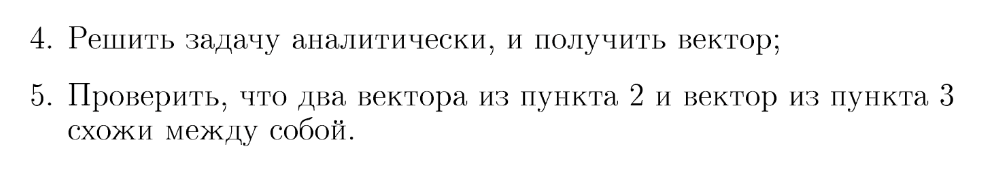
\includegraphics{tables/3.png}

\section{Выводы и анализ работы}

 Мы используем фотон, как средство передачи информации.
 
 С помощью полуволновых пластинок, которые определяют базис, и поляризационных разделительных кубов, которые отражают свет с вертикальной поляризацией и пропускают с горизонтальной, при отправлении фотона можем получить определенный результат, который может быть перехвачен.

Перехватчик -- собранная Алиса и Боб, но в обратной последовательности.

Если Ева угадывает базис, то получает всю информацию Алисы незамеченно. 
При неудачной попытке на один из детекторов приходит неверный бит, и Ева отправит сигнал Бобу. При дальнейшей проверке базисов Алисы и Боба это будет заметно с вероятностью 25\%. Тогда будет произведена замена ключа.


\end{document}
